\documentclass[referat]{SCWorks}
% параметр - тип обучения - одно из значений:
%    spec     - специальность
%    bachelor - бакалавриат (по умолчанию)
%    master   - магистратура
% параметр - форма обучения - одно из значений:
%    och   - очное (по умолчанию)
%    zaoch - заочное
% параметр - тип работы - одно из значений:
%    referat    - реферат
%    coursework - курсовая работа (по умолчанию)
%    diploma    - дипломная работа
%    pract      - отчет по практике
% параметр - включение шрифта
%    times    - включение шрифта Times New Roman (если установлен)
%               по умолчанию выключен
\usepackage{preamble}

%\usepackage{titlesec}
\setcounter{secnumdepth}{4}
%\titleformat{\paragraph}
%{\normalfont\normalsize}{\theparagraph}{1em}{}
%\titlespacing*{\paragraph}
%{35.5pt}{3.25ex plus 1ex minus .2ex}{1.5ex plus .2ex}

\titleformat{\paragraph}[block]
{\hspace{1.25cm}\normalfont}
{\theparagraph}{1ex}{}
\titlespacing{\paragraph}
{0cm}{2ex plus 1ex minus .2ex}{.4ex plus.2ex}

%~--------------------------------------------------------------------------%


\usepackage[T2A]{fontenc}
\usepackage[utf8]{inputenc}
\usepackage{graphicx}
\graphicspath{ {./images/} }
\usepackage{tempora}

\usepackage[sort,compress]{cite}
\usepackage{amsmath}
\usepackage{amssymb}
\usepackage{amsthm}
\usepackage{fancyvrb}
\usepackage{listings}
\usepackage{listingsutf8}
\usepackage{longtable}
\usepackage{array}
\usepackage[english, russian]{babel}

%\usepackage[colorlinks=true]{hyperref}
\usepackage{url}
\usepackage{ulem}

\usepackage{underscore}
\usepackage{setspace}
\usepackage{indentfirst} 
\usepackage{mathtools}
\usepackage{amsfonts}
\usepackage{enumitem}
\usepackage{tikz}
\newcommand{\eqdef}{\stackrel {\rm def}{=}}
\newcommand{\specialcell}[2][c]{%
\begin{tabular}[#1]{@{}c@{}}#2\end{tabular}}

\renewcommand\theFancyVerbLine{\small\arabic{FancyVerbLine}}

\newtheorem{lem}{Лемма}

\begin{document}

% Кафедра (в родительном падеже)
\chair{теоретических основ компьютерной безопасности и криптографии}

% Тема работы
\title{Коллаборативная фильтрация в рекомендательных системах}

% Курс
\course{5}

% Группа
\group{531}

% Факультет (в родительном падеже) (по умолчанию "факультета КНиИТ")
\department{факультета КНиИТ}

% Специальность/направление код - наименование
%\napravlenie{09.03.04 "--- Программная инженерия}
%\napravlenie{010500 "--- Математическое обеспечение и администрирование информационных систем}
%\napravlenie{230100 "--- Информатика и вычислительная техника}
%\napravlenie{231000 "--- Программная инженерия}
\napravlenie{10.05.01 "--- Компьютерная безопасность}

% Для студентки. Для работы студента следующая команда не нужна.
\studenttitle{cтудентки}

% Фамилия, имя, отчество в родительном падеже
\author{Ивановой Ксении Всладиславовны}

%Научный руководитель (для реферата преподаватель проверяющий работу)
\satitle{Доцент} %должность, степень, звание
\saname{И. И. Слеповичев}

% Руководитель практики от организации (только для практики,
% для остальных типов работ не используется)
%\patitle{к.ф.-м.н.}
%\paname{М.~Б.~Абросимов}

% Семестр (только для практики, для остальных
% типов работ не используется)
%\term{8}

% Наименование практики (только для практики, для остальных
% типов работ не используется)
%\practtype{преддипломная}

% Продолжительность практики (количество недель) (только для практики,
% для остальных типов работ не используется)
%\duration{4}

% Даты начала и окончания практики (только для практики, для остальных
% типов работ не используется)
%\practStart{30.04.2019}
%\practFinish{27.05.2019}

% Год выполнения отчета
\date{2024}

\maketitle

% Включение нумерации рисунков, формул и таблиц по разделам
% (по умолчанию - нумерация сквозная)
% (допускается оба вида нумерации)
% \secNumbering

%-------------------------------------------------------------------------------------------
\tableofcontents

\intro

Одна из интересных тем современного мира, которая стоит на стыке информационных технологий и маркетинга,
не дающая уснуть ночью, подкидывая нам интересные видео, и помогающая тратить наши деньги, предлагая товары,
которые нам <<могут понравиться>>, тема рекомендательных систем. 

Сейчас, в период информационной зависимости, вопрос 
<<что надеть>>, смещается более актуальным <<что посмотреть>>, а продвижение товара преобразуется из rтелевизионно"=зомбирующей рекламы совершенно ненужных вам вещей в предложения купить товары с оценкой 5 звезд 
из 5. Умные алгоритмы рекомендаций товаров на основе каких-то действий или признаков покупателя помогают как бизнесу, 
так и потребителям. Одним из таких методов является коллаборативная фильтрация, о которой и пойдет речь. 


\section{Метод коллаборативная фильтрации}
К коллаборативной (совместной) фильтрации относятся те методы и
алгоритмы, которые основываются на данных о предыдущих сеансах работы пользователей с этой же
системой. 

Общая черта всех методов коллаборативной фильтрации это то, что основой создания
рекомендаций является пересечение оценочных мер популярности того или иного объекта.
Мерой оценивания объекта можно выбрать не только данные, которые предоставил нам сам пользователь, используя функционал сервиса: отметка звездочкой или оценка объекту,
но также можно учитывать данные, которые пользователь предоставляет неосознанно: 
количество просмотров, время посещения, количество переходов, потраченная сумма \cite{smolenchuk}.

\begin{figure}[H]
  \centering
  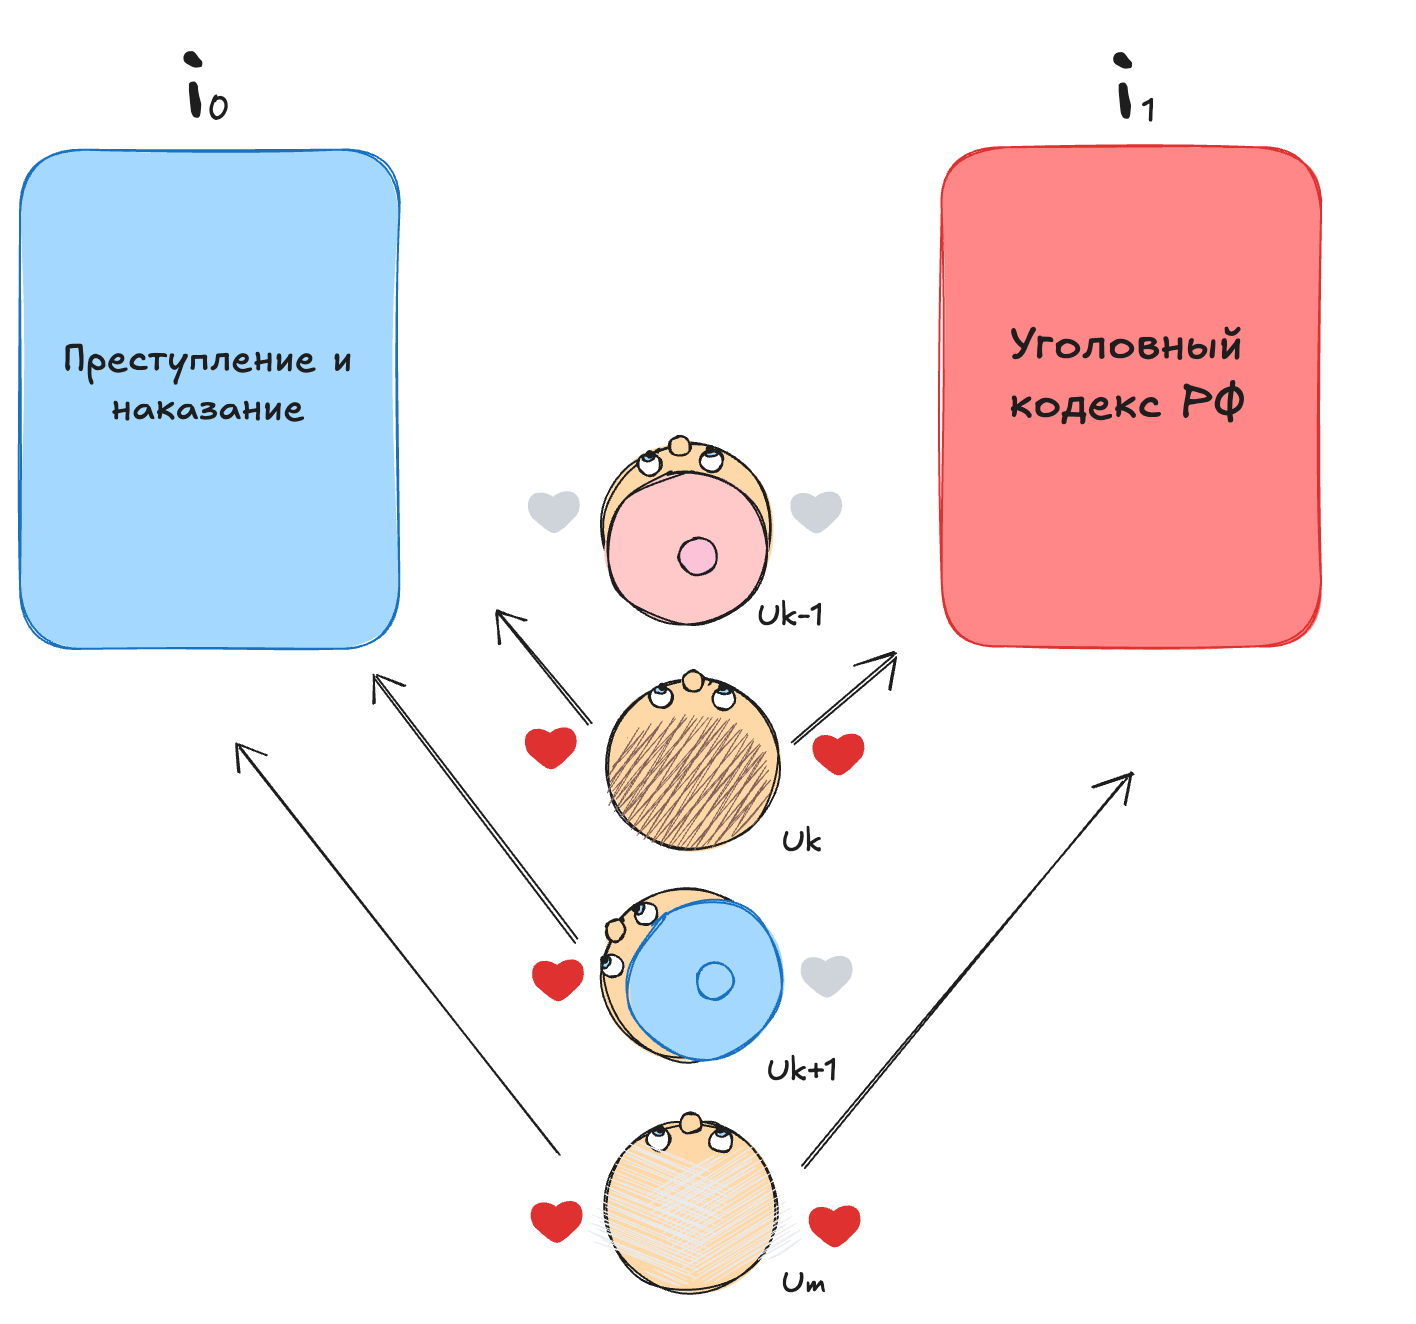
\includegraphics[width=0.7\textwidth]{./2.png}
  \caption{}
\end{figure}

Посмотрим пример тривиальной рекомендации для рисунка 1.
Формируется матрица предпочтений (user-item matrix), которая отражает взаимодействие 
пользователей с различными предметами, в нашем случае она отражает понравилась ли 
пользователю книга. Видим, что пользователем и $u_k$, $u_{k+1}$, $u_m$, понравились одинаковые книги, таких пользователей будем называть <<окрестностями>> или <<коллаборацией>>, обозначим за $U(i_0)$. 
Предполагаем, что книга $i_0$ похожа на $i_1$, потому что она понравилась похожим людям, множество таких книг образуется формулой (1), поэтому рекомендуем пользователю $u_{k+1}$ 
прочитать книгу $i_1$. Интересный факт, что данный принцип  <<клиенты купившие предмет A, также купили предмет B>>, для потребительских манипуляций первым придумали использовать у себя нв страницах
Amazon.com, слоган используется до сих пор, хотя алгоритмы подбора рекомендации используют другие принципы.

\[ I(i_0) = \{ i \in I |  sim(i_0, i_1) = \vert \frac{U(i_0)\cap U(i_1)}{U(i_0) \cup  U(i_1)}  \vert \}, \eqno(1) \]
где $sim(i_0, i_1)$ "--- мера оценивания близости двух книг $i_0$ и $i_1$.

Несложно оценить, что метод имеет ряд недостатков:
\begin{enumerate}
  \item Рекомендации предлагают самые популярные товары;
  \item Не учитываются интересы конкретного пользователя $u_i$;
  \item Новый товар никому не рекомендуется;
  \item Нужно хранить матрицу предпочтений.
  \end {enumerate}

Рассмотрим два больших вида подходов в коллаборативной фильтрации, а также их выигрышные и наоборот стороны.

\subsection{Корреляционные модели}
Корреляционные модели или на английском языке <<Memory"=Based Collaborative Filtering>>.
В моделях этого вида для построения прогнозов используется выявление разного рода 
корреляций между пользователями на основе матрицы соответствия оценок пользователей и объектов.

Отличающие особенности:
\begin{itemize}
  \item Хранение всей исходной матрицы данных;
  \item Сходство клиентов "--- это корреляция строк;
  \item Сходство объектов "--- это корреляция столбцов.
\end{itemize}

Описанный в предыдущей главе пример также относится к коллаборативной фильтрации, только в самом 
наивном ее представлении, в основном корреляционные модели делятся на два подхода "--- <<От клиента>> и <<От предмета>>.

\subsubsection{От клиента}
В данном подходе немного меняется формулировка фразы <<клиенты купившие предмет A, также купили предмет B>> на <<клиенты похожие на 
Вас, также купили предмет B>>. Если рассматривать матрицу отношений то <<От клиента>> означает, 
что корреляцию будем искать между строками матрицы, т.е пользователями \cite{beamer}.

Для простоты представим, что пользователь
оценивает понравилась музыкальная группа или нет, таким образом в матрице, если группа понравилась "--- на пересечении пользователя и группы ставится красное сердце, 
если группа известна, но особых чувств не вызвала "--- пустое сердце, если данный объект еще не попадался пользователю "--- пустая ячейка.
Матрица R показана на рисунке 2.

\begin{figure}[H]
  \centering
  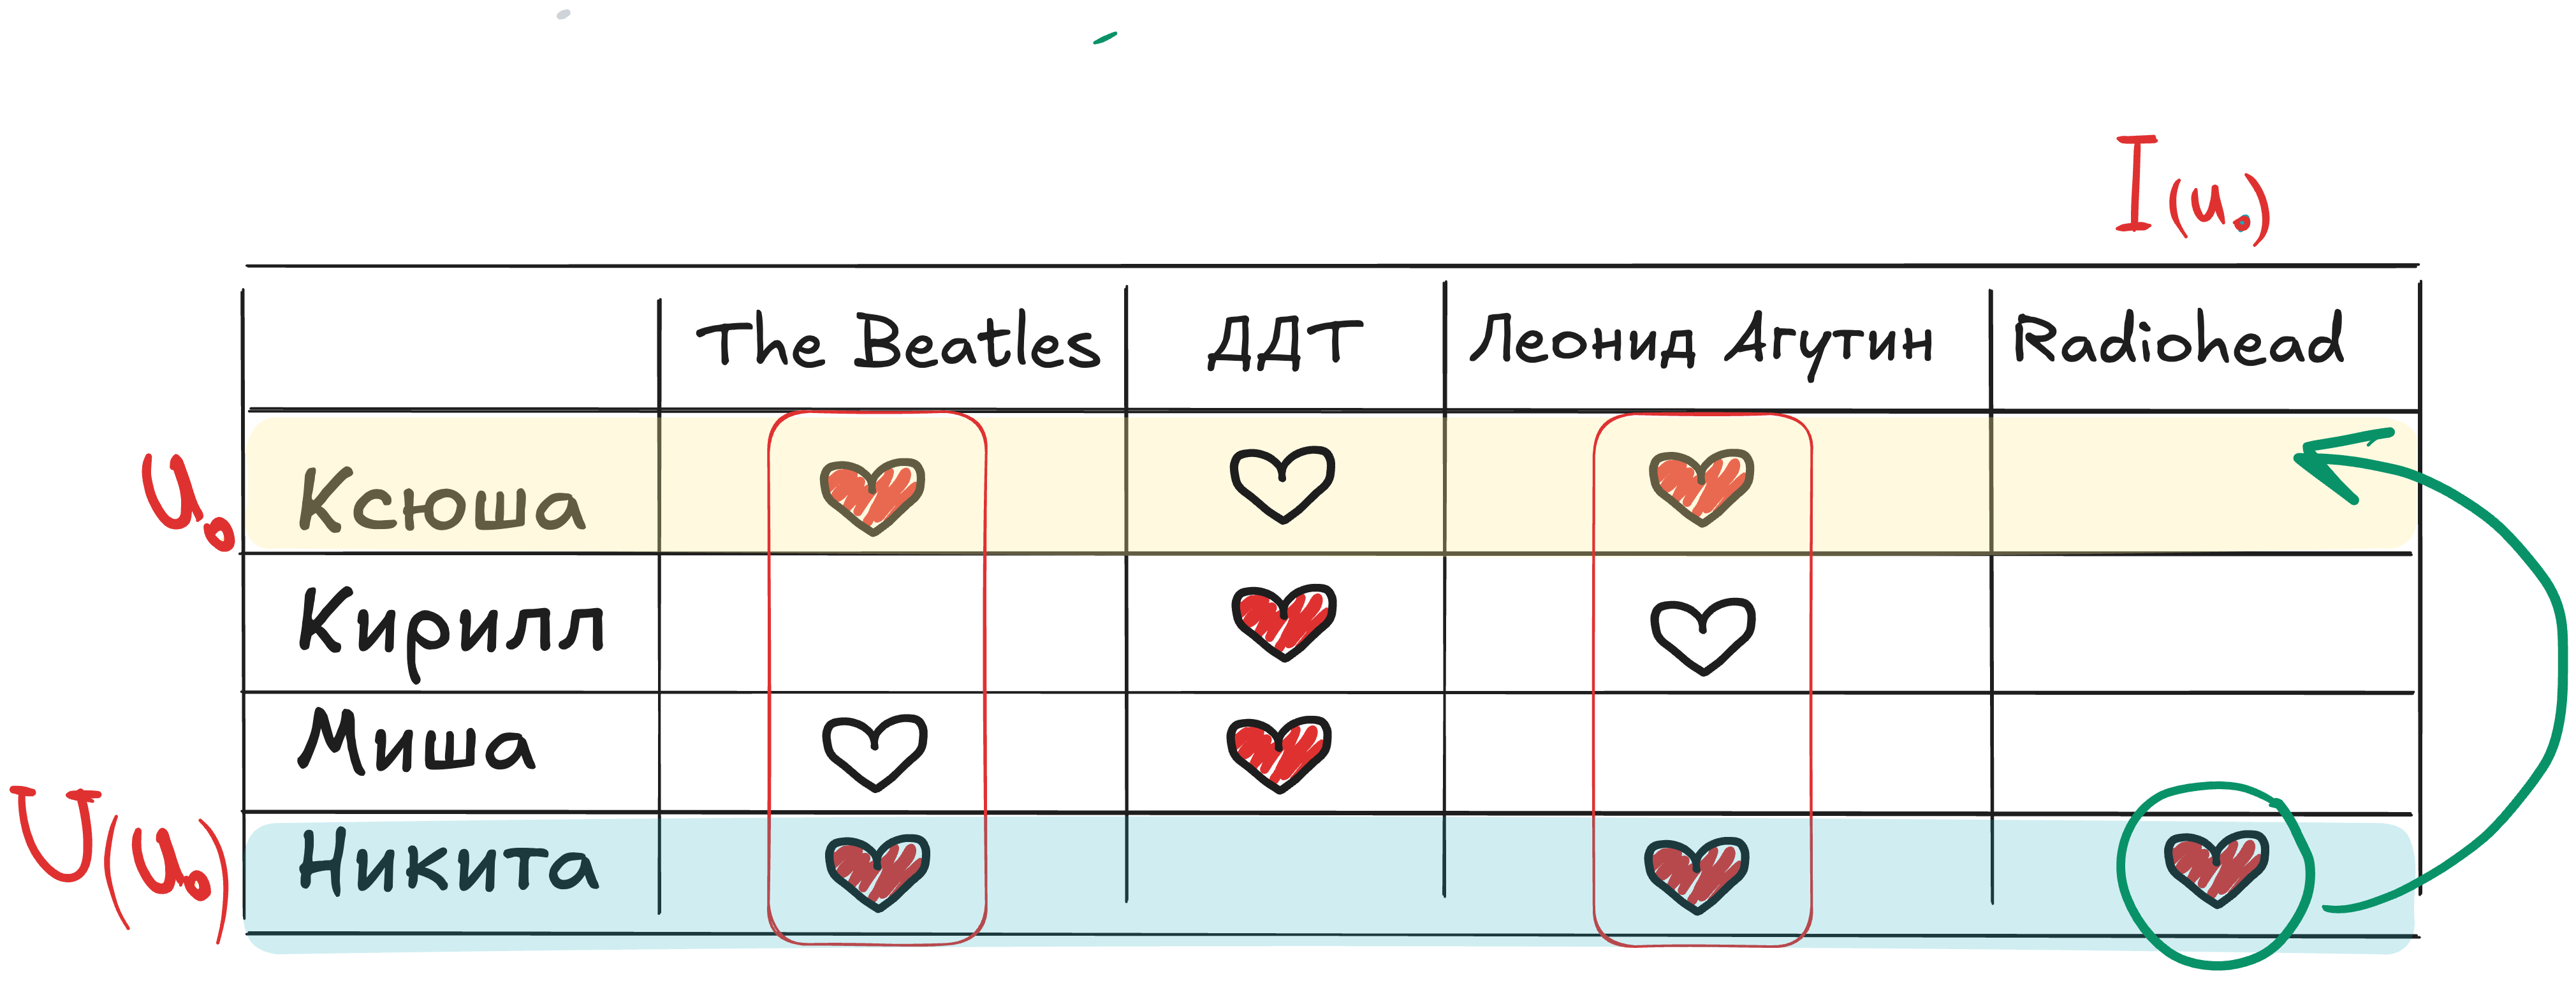
\includegraphics[width=1\textwidth]{./3.png}
  \caption{}
\end{figure}

Коллаборация пользователей, близких по интересам зададим формулой (2).
\[ U(u_0) = \{ u \in U | sim(u_0, u) >\alpha \}, \eqno(2) \]
где $sim(i, i_0)$ "--- мера оценивания близости двух пользователей $u$ и $u_0$.

А множество схожих объектов, которые можно отсортировать по убыванию некоторой функции $B(i)$, а далее предложить 
пользователю можно выразить формулой (3).
\[ I(i_0) = \{ i \in I |  B(i) = \vert \frac{U(u_0)\cap U(i)}{U(u_0) \cup U(i)}  \vert \}, \eqno(3) \]
где $U(i) = \{ u \in U | r_{u, i}\neq \varnothing \}$ . \\


Рассмотрим алгоритм, который предсказывает оценкy для объектов, еще неоцененных данным пользователем:\\
\begin{figure}[H]
  \centering
  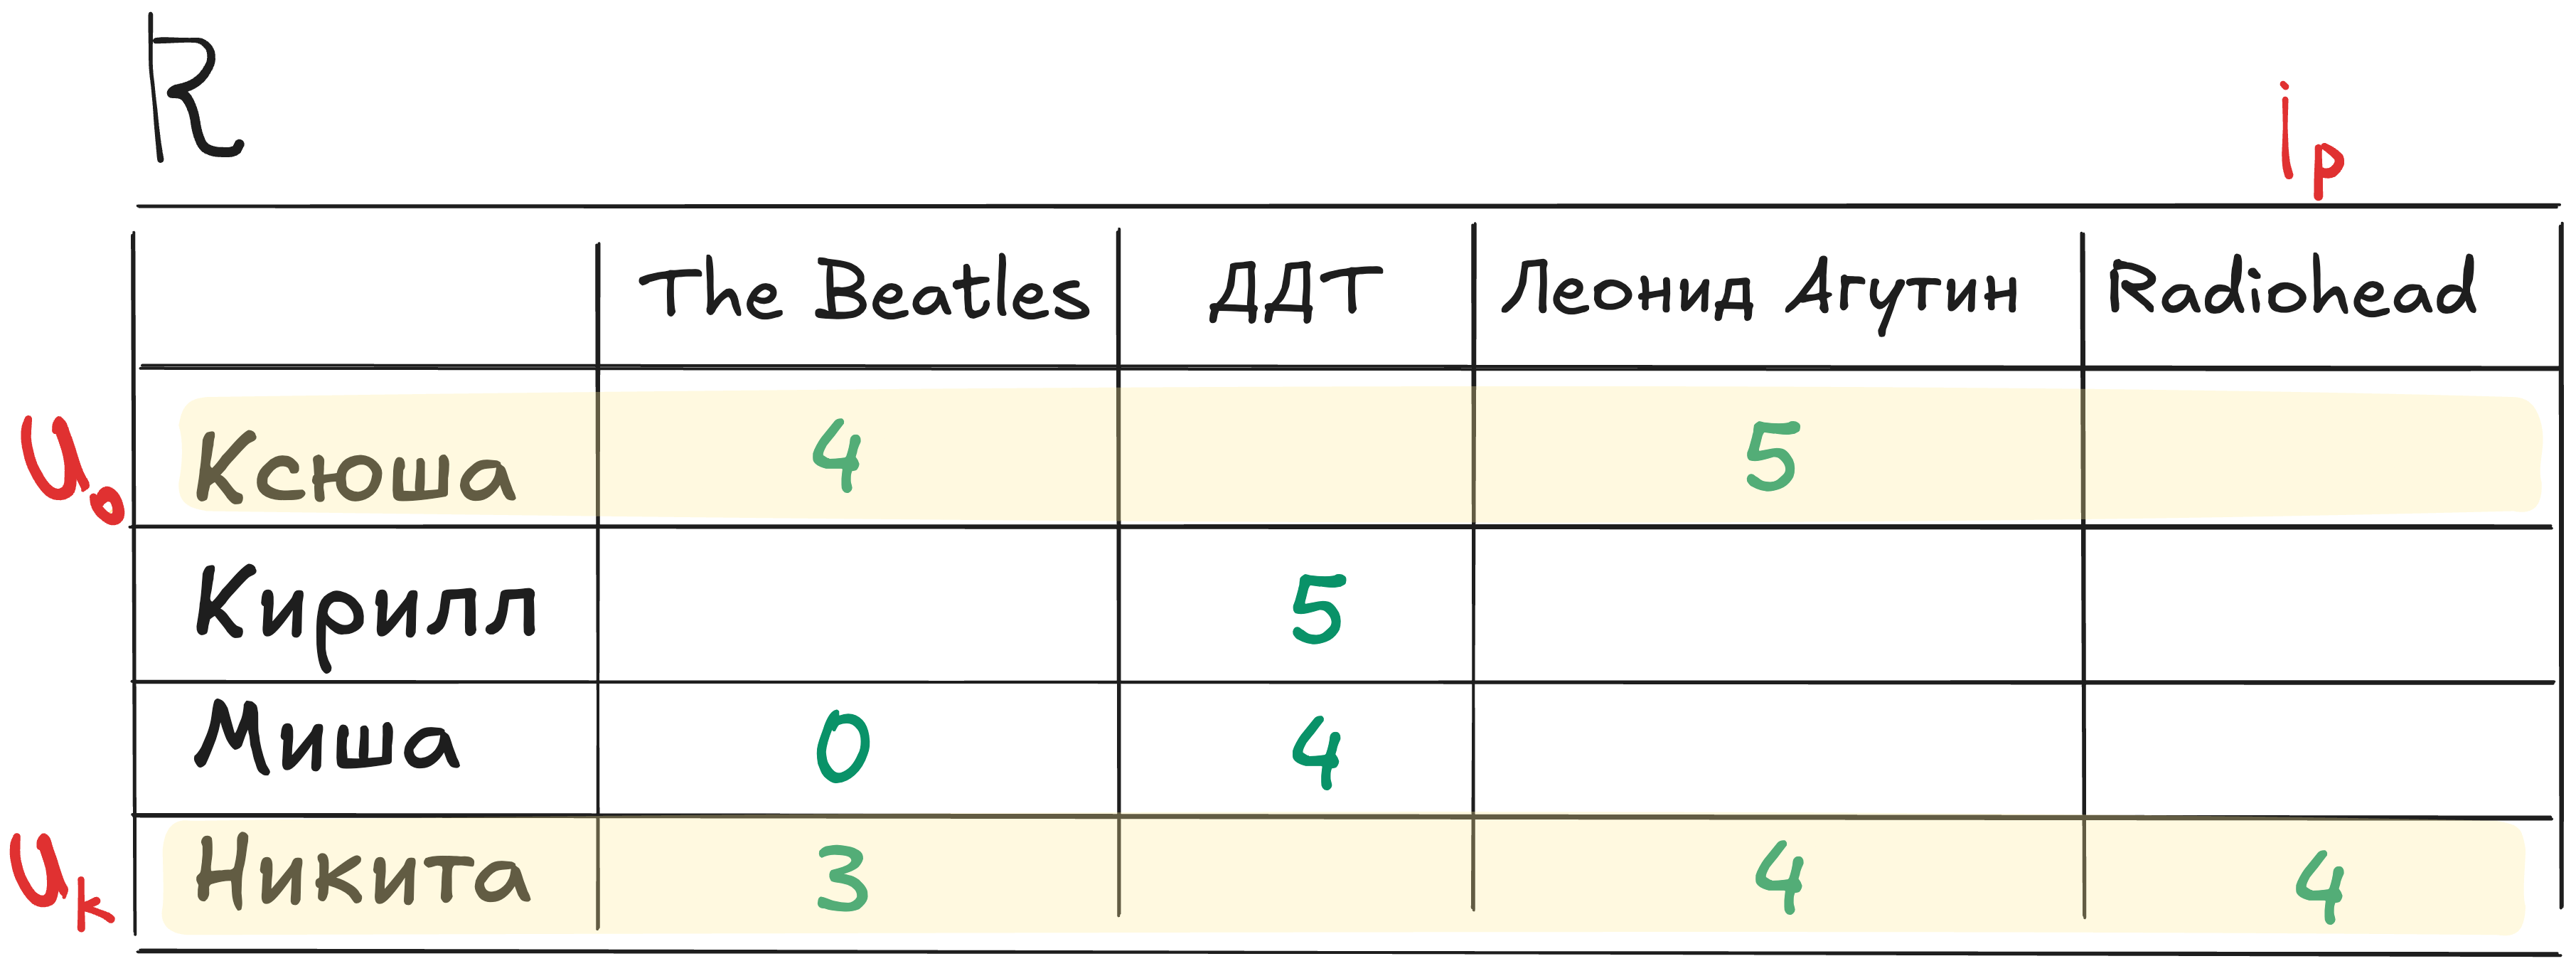
\includegraphics[width=1\textwidth]{./6.png}
  \caption{}
\end{figure}

Шаг1. Немного изменим предыдущий рисунок, пусть вместо <<сердечек>>, пользователь выставляет числовые
оценки, рассмотрим рисунок 3. 
Вычислим близость строк в матрице R, будем учитывать только тех пользователей, которые оценивали объекты. Есть много видов
метрик, которые можно использовать, проще всего будет взять косинусное расстояние формула (4).
\[ sim(u_0, u_k) =  \frac{\sum_{i = 1}^{m} r_{u_0,i} \cdot r_{u_k,i }}{\sqrt{\sum_{i = 1}^{m} r_{u_0,i}} \cdot \sqrt{{\sum_{i = 1}^{m} r_{u_k,i }}}},  \eqno(4) \]
где $sim(u_0, u_k)$ близость пользователей $u_0$ и $u_k$, $r_{u_0,i}, r_{u_k,i }$ "--- значения матрицы $R$.

Немного про метрики,  пусть у нас есть три вектора оценок от пользователей $a=(5, 5, 2), b = (2, 2, 0), c = (0, 0, 2)$.
Если мы возьмем в качестве метрики евклидово расстояние, то наиболее 
близкими будут вектора $b$ и $c$ т.к их нормы ближе по значению по сравнению с $a$, в отличие от косинусной метрики, 
где $b$ и $c$ вообще не имеют общих оценок от пользователей, поэтому ближе будут  $a$ и $b$. 
Поэтому при выборе метрики нужно учитывать специфику задачи.


Шаг2. После того как мы посчитали близости между пользователями, все пользователи сортируются по убыванию меры близости,
нужно выбрать множество, назовем его $K$, похожих на $u_0$. Можно выбрать и всех пользователей, но тогда непохожие пользователи 
будут сильно влиять на точность предсказания оценки, также это будет служит дополнительным объемом данных для вычислений на 3 шаге.

Лучше выбрать какое-то пороговое значение, которое будет приблизительно достоверно оценивать <<похожесть>>, обычно выбирается целая константа.
\\

Шаг3. Вычисляем приблизительную оценку, которую пользователь $u_0$ поставил бы объекту $i_p$, формула (5).

\[ p(u_0, i_p) = \overline{r}_{u_0} + \frac{\sum_{u\in K} (r_{u_0,i_p} - \overline{r}_{u_0})\times sim(u_0, u_k)}{\sum_{u\in K}  \vert sim(u_0, u_k) \vert } ,   \eqno(5) \]
где $p(u_0, i_p)$ "--- предсказываемая оценка, правое слагаемое "--- среднее отклонение оценки других пользователей из $K$ для объекта $i_p$ от их реальной оценки.

Так как для каждого пользователя понятие <<рейтинг>> очень субъективное, кто-то поставит хорошему фильму оценку <<5>>, а кто-то оценку <<4>>, ибо есть идеал и он недостижим, 
чтобы сгладить такие различия между пользователями, в формуле (5) сначала вычитается, а потом добавляется средняя оценка пользователя $r_{u_0}$. Сама же формула
носит название <<непараметрическая регрессия Надарайя"--~Ватсона>> или <<формула ядерного сглаживания>>.

Часть недостатков удалось устранить, но все также остаются следующие:
\begin{enumerate} 
  \item \sout{Рекомендации предлагают самые популярные товары};
  \item \sout{Не учитываются интересы конкретного пользователя $u_i$};
  \item Новый товар никому не рекомендуется;
  \item Нужно хранить матрицу предпочтений;
  \item Нечего рекомендовать нетипичным пользователям.
\end {enumerate}

\subsubsection{От предмета}
Данный метод характеризуется фразой: <<вместе с объектами которые покупал пользователь $U_o$, также часто покупают...>>.
Используя этот метод, при рекомендации мы учитываем некоторые действия которые уже совершил пользователь. В отличие от предыдущего метода
корреляция ищется между столбцами матрицы R, т.~е рассматриваются музыкальные группы похожие на те, что пользователе уже оценил, рисунок (4). 

\begin{figure}[H]
  \label{fig:item}
  \centering
  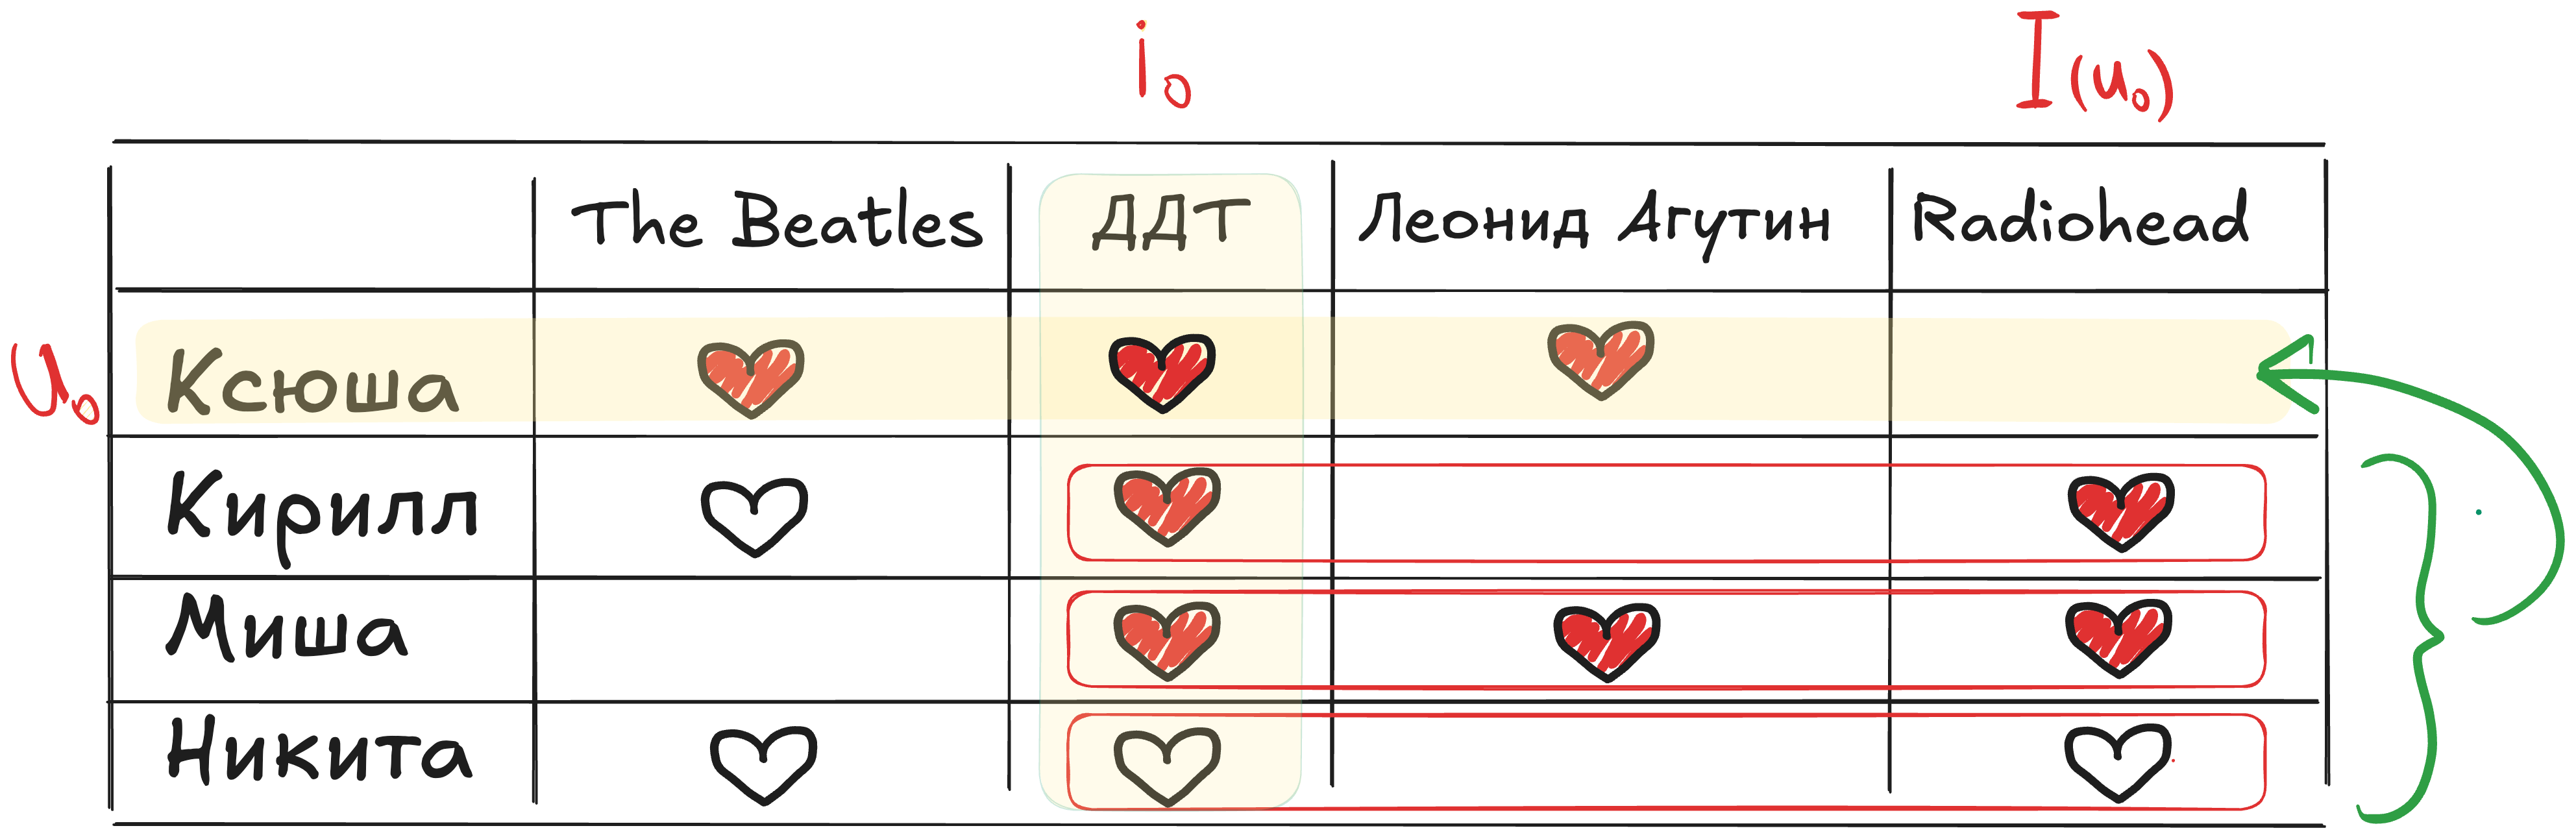
\includegraphics[width=1\textwidth]{./4.png}
  \caption{Таблица соответствия пользователей их оценкам для музыкальных групп.}
\end{figure}
Множество похожих объектов можно выразить формулой (6).
\[ I(u_0) = \{ i \in I | \exists  i_0: r_{u_0, i_0}\neq \varnothing \wedge  B(i) = sim(i, i_o) >\alpha \}, \eqno(6) \]
где $sim(i, i_0)$ "--- мера оценивания близости двух книг $i$ и $i_0$.\\
Если рассматривать алгоритм работы, он очень похож на алгоритм <<От клиента>>.\\
Шаг1. Для каждого объекта $i_p$ вычисляется на сколько он похож на объект $i_k$ для которого предсказывается оценка, формула (7).

\[ sim(i_k, i_p) =  \frac{\sum_{i = 1}^{n} r_{i_k,i} \cdot r_{i_p,i }}{\sqrt{\sum_{i = 1}^{m} r_{i_k, i}} \cdot \sqrt{{\sum_{i = 1}^{n} r_{i_p,i }}}},   \eqno(7) \]
где $sim(i_k, i_p)$ близость объектов $i_k$ и $i_p$, $r_{i_k,i}, r_{i_p,i}$ "--- значения матрицы $R$.\\
Шаг2. Выбирается множество объектов наиболее похожих на $i_k$.\\
Шаг3. Предсказывается оценка для выбранных на шаге 2 объектов, используя формулу (8).
\[ p(u_0, i_k) =  \frac{\sum_{i_k\in K} r_{u_0,i_p} \times sim(i_k, i_p)}{\sum_{i_k\in K}  \vert sim(i_k, i_p) \vert },    \eqno(8) \] 
где $p(u_0, i_p)$ "--- предсказываемая оценка, правое слагаемое "--- среднее отклонение оценки других пользователей из $K$ для объекта $i_p$ от их реальной оценки.

Уже интереснее, но все еще есть некоторые минусы:
\begin{enumerate} 
  \item Рекомендации предлагают самые популярные товары (нет коллаборативности);
  \item \sout{Косвенно учитываются интересы конкретного пользователя};
  \item Новый товар никому не рекомендуется;
  \item Нужно хранить матрицу предпочтений;
  \item \sout{Нечего рекомендовать нетипичным пользователям}.
  \end {enumerate}  

\subsection{Латентные модели}
Латентные модели или на английском <<Latent Models for Collaborative Filtering>>.
Для каждого пользователя или объекта будем рассматривать не вектор
его взаимодействий с соответствующими элементами рекомендательной системы, 
а некий профиль "--- вектор, который описывает объект
или пользователя в каком-то пространстве, размерность которого, как правило, 
много меньше размерностей исходной матрицы R.

Также можем представить это в виде некоторого пространства рисунок 5, где пользователи
и объекты размещены в плоскости тегов, исходя из тегов в их профилях, тогда можем видеть, что 
некоторые субъекты ближе к каким-то объектам и это можно использовать для создания рекомендаций.

\begin{figure}[H]
  \centering
  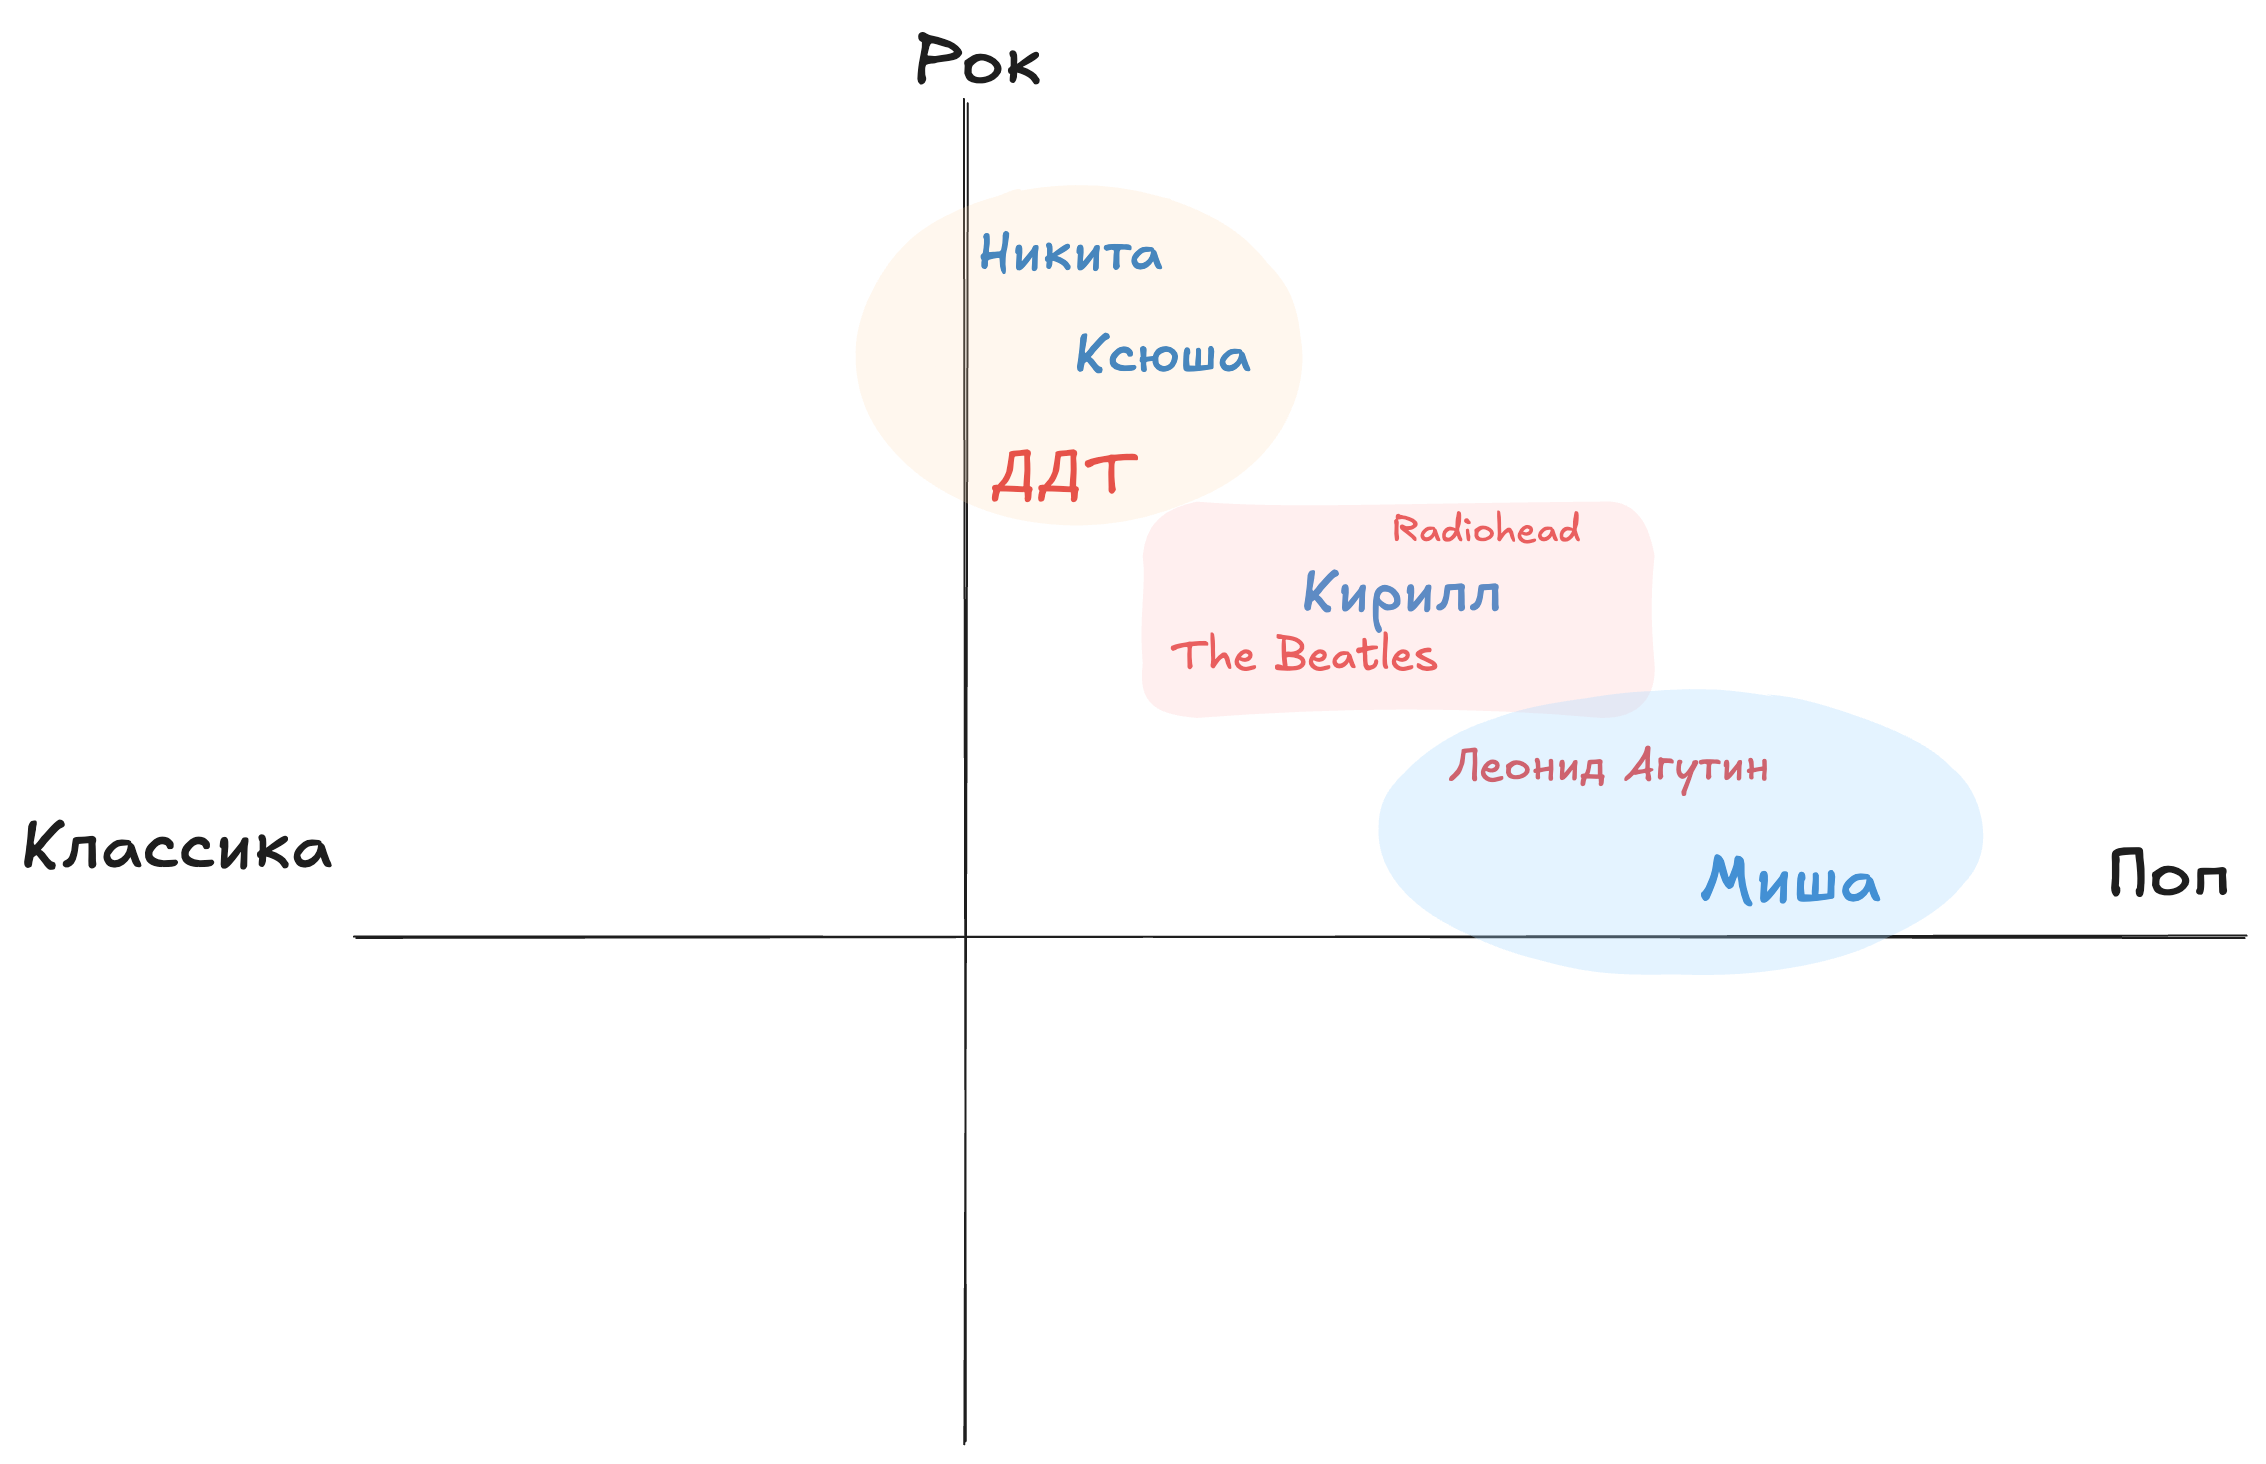
\includegraphics[width=0.8\textwidth]{./7.png}
  \caption{}
\end{figure}


Некоторые особенности:
\begin{itemize}
  \item Профиль "--- это вектор скрытых характеристик;
  \item Хранение профилей вместо хранения матрицы данных;
  \item Сходство клиентов и объектов "--- это сходство их профилей.
\end{itemize}
Рассмотрим некоторые типы идей латентных моделей.

\subsubsection{Ко-кластеризация}
Идея в том, что нам нужно разделить множество клиентов и объектов по кластерам и найти соответствия для
кластеров объектов и пользователей.
Бывает жесткая и мягкая кластеризации. Жесткая "--- приписываем пользователям конкретные кластеры, со степенью принадлежности либо 0 либо 1, например <<Никита любит рок>>.
В мягкой кластеризации степень принадлежности величина вещественная, может быть в промежутке значений от 0 до 1, например <<Никита относится к року с мерой 0.8>>

В качестве примера, можем рассмотреть алгоритм под названием <<Латентное размещение Дирихле (LDA)>>
Латентное размещение Дирихле (LDA) "--- это вероятностная модель, разработанная для моделирования тем в коллекциях документов. 
Она основана на предположении, что каждый документ может быть представлен как смесь различных тем, а каждая тема связана с распределением слов.

Алгоритм LDA можно разбить на несколько шагов:

Шаг1. Для применения LDA необходимо заранее определить количество тем, которые
вы хотите выделить. Это может быть достаточно сложной задачей, и выбор зависит 
от конкретных характеристик данных, также нужно выбрать параметры модели.

Шаг2. Подготовка данных. Документы преобразуются в числовое представление, например, с помощью TF"=IDF матриц (показывает, сколько раз каждое слово встречается в каждом документе).

Шаг3. Инициализируются распределения тем для документов и распределения слов для тем.

Шаг4. Происходит обучение, итеративно обрабатывается тексты, чтобы определить, какие темы присутствуют 
в документах и какие слова связаны с каждой темой. 
\begin{itemize}
  \item Для каждого слова в каждом документе вычисляется вероятность принадлежности к каждой теме, используя текущие распределения тем и слов;
  \item На основе вероятностей слов в темах и вероятностей тем в документах пересчитываются распределения тем и слов;
\end{itemize}

Алгоритм старается максимизировать вероятность появления слов в каждой теме и вероятность наличия тем в каждом документе.
По окончании итераций можно получить распределения тем для каждого документа и распределения слов для каждой темы.\\
Некоторые недостатки:
\begin{itemize}
  \item Определение оптимального количества тем может быть сложной задачей и требует экспериментов;
  \item Результаты могут сильно зависеть от исходных параметров и инициализации;
  \item Необходима тщательная предобработка данных, включая удаление стоп-слов и другие шаги.
\end{itemize}

\subsubsection{Матричная факторизация}
Была такая известная история про приз от Netflix. В 2006 году компания пообещала выплатить 1 млн разработчикам, которые 
смогут улучшить эффективность её алгоритма рекомендации фильмов минимум на $10\%$.
В конкурсе, длившемся почти три года, участвовали десятки тысяч команд со всего мира. В итоге выиграла BellKor Pragmatic Chaos,
в которую вошли учёные из американской ATT Labs и австрийской Commendo Research Consulting. Она даже немного перевыполнила план "--- эффективность алгоритма улучшилась на $10,05\%$.
Решение победившей команды использовало матричную факторизацию, а сейчас ее используют в своих системах почти все гиганты 
интернет пространства: Amazon, Spotify, YouTube. Задача поиска матриц $U$ и $I$, таких что $R = U \cdot I$

\begin{figure}[H]
  \centering
  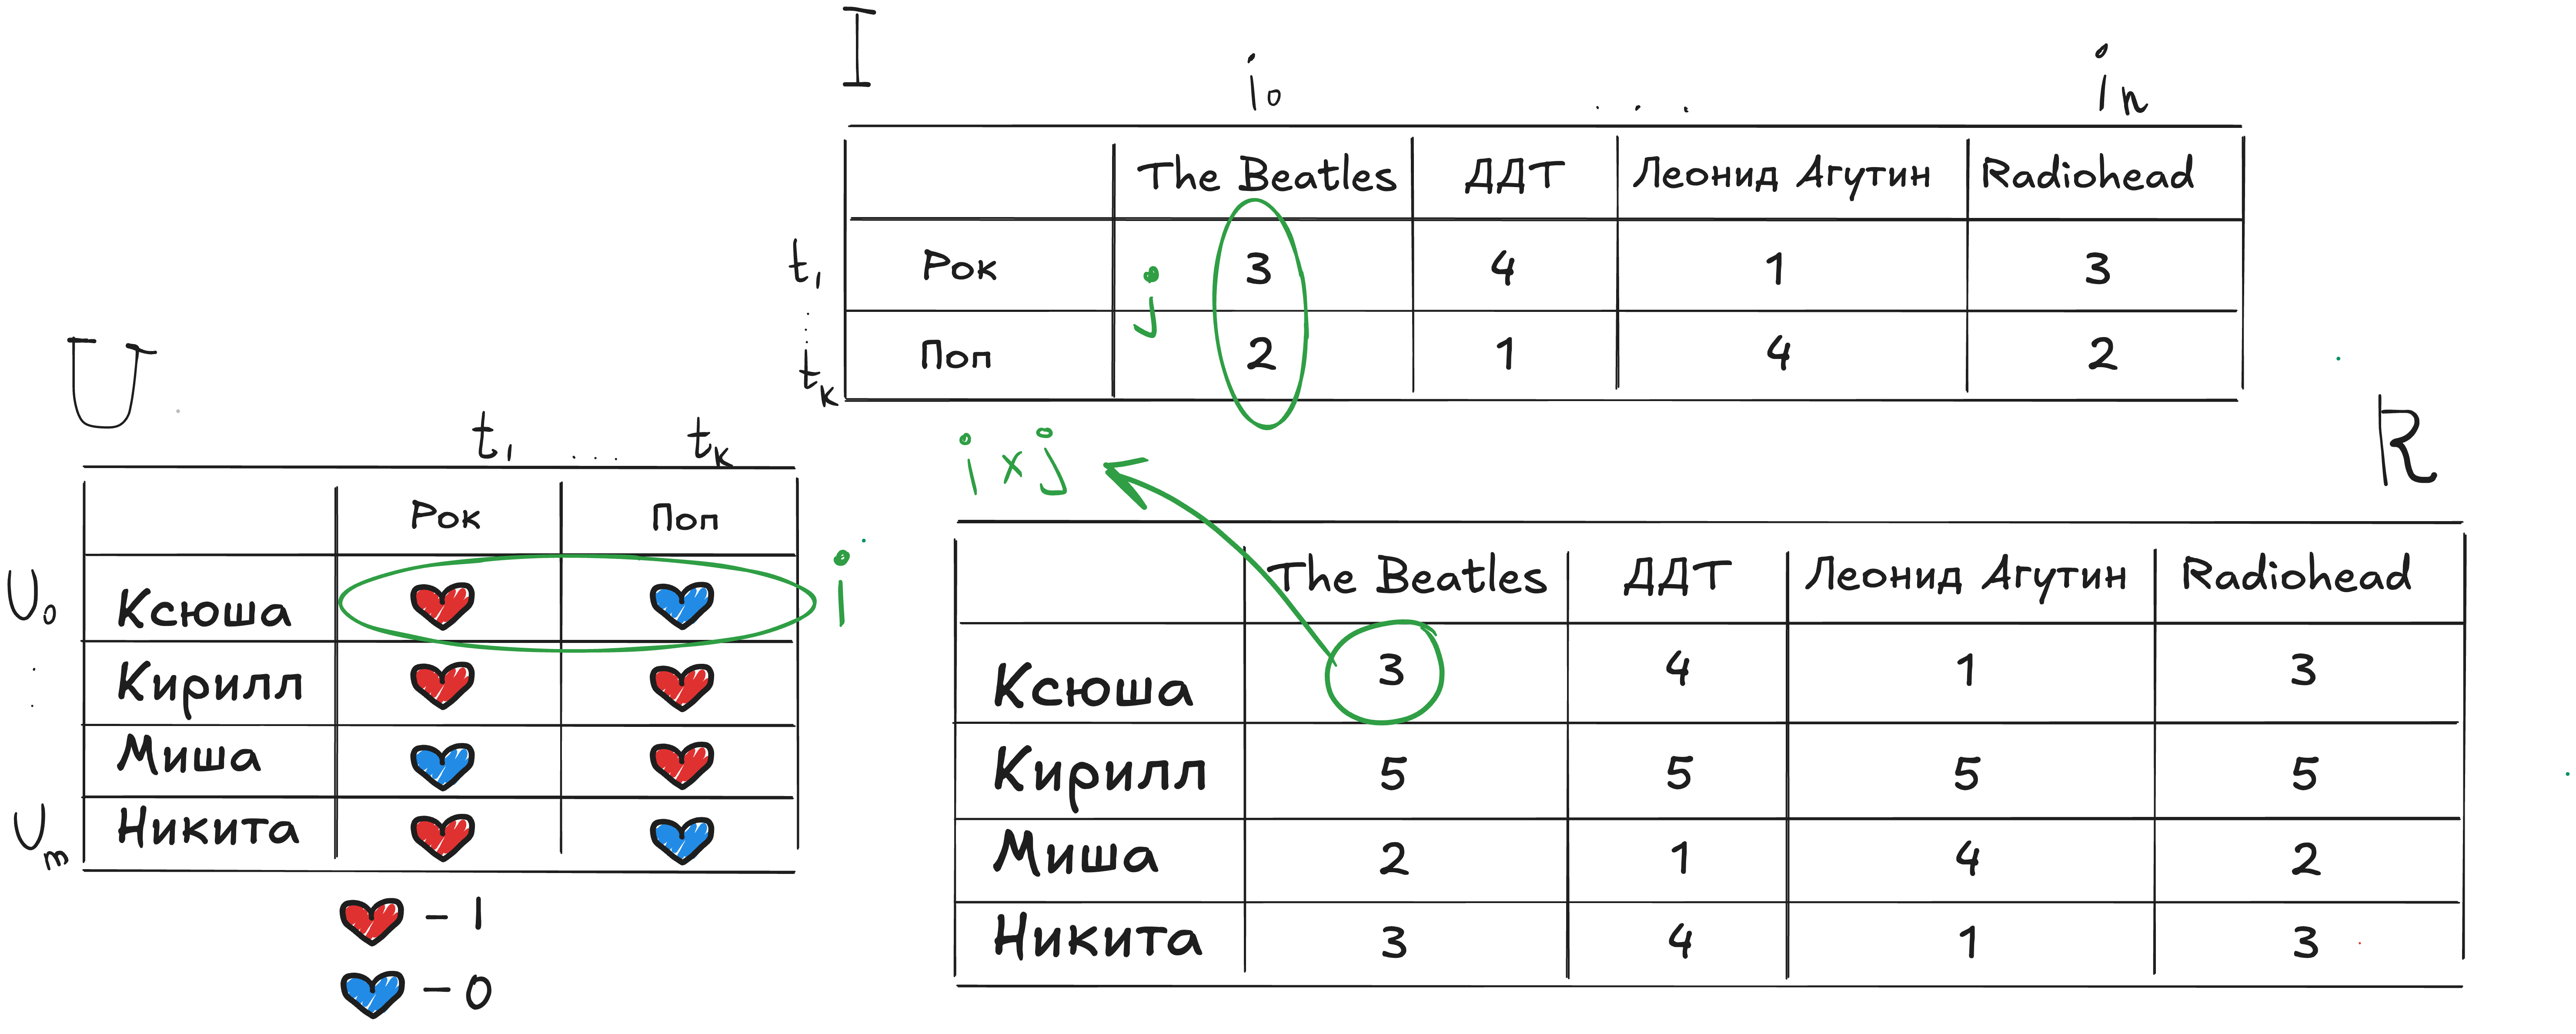
\includegraphics[width=1\textwidth]{./5.png}
  \caption{}
\end{figure}


\[ TF(x, D) = \frac{freq(x, D)}{max_{y \in D}freq(y, D)}   \eqno(4) \]
где $freq(x, D)$ количество слов $x$ в документе $D$.

\[ IDF(x) = \frac{N}{n(x)}   \eqno(4) \]
где $N$ количество документов наборе, $n(x)$ "--- количество документов, в которых встречается $x$.


Т.к модель у нас латентная, мы будем хранить две матрицы "--- пользователи\,--\,теги и теги\,--\,объекты (матрица $U$ показывает 
относится ли пользователь к какому-то тегу, а вторая $I$ на сколько музыкальная группа соответствует тегу по 5 бальной шкале),
тогда мы можем просчитать рейтинг, который пользователь может поставить объекту, можно выразить это как скалярное произведение
строки $i$ и столбца $j$.
Но предположим нам нужно научиться предсказывать оценки, тогда мы можем обучить нейронную сеть, корректируя 
неизвестные оценки в матрицах $U$ и $I$, минимизируя функцию ошибки от матрицы $R$ и $R'$
\begin{figure}[H]
  \centering
  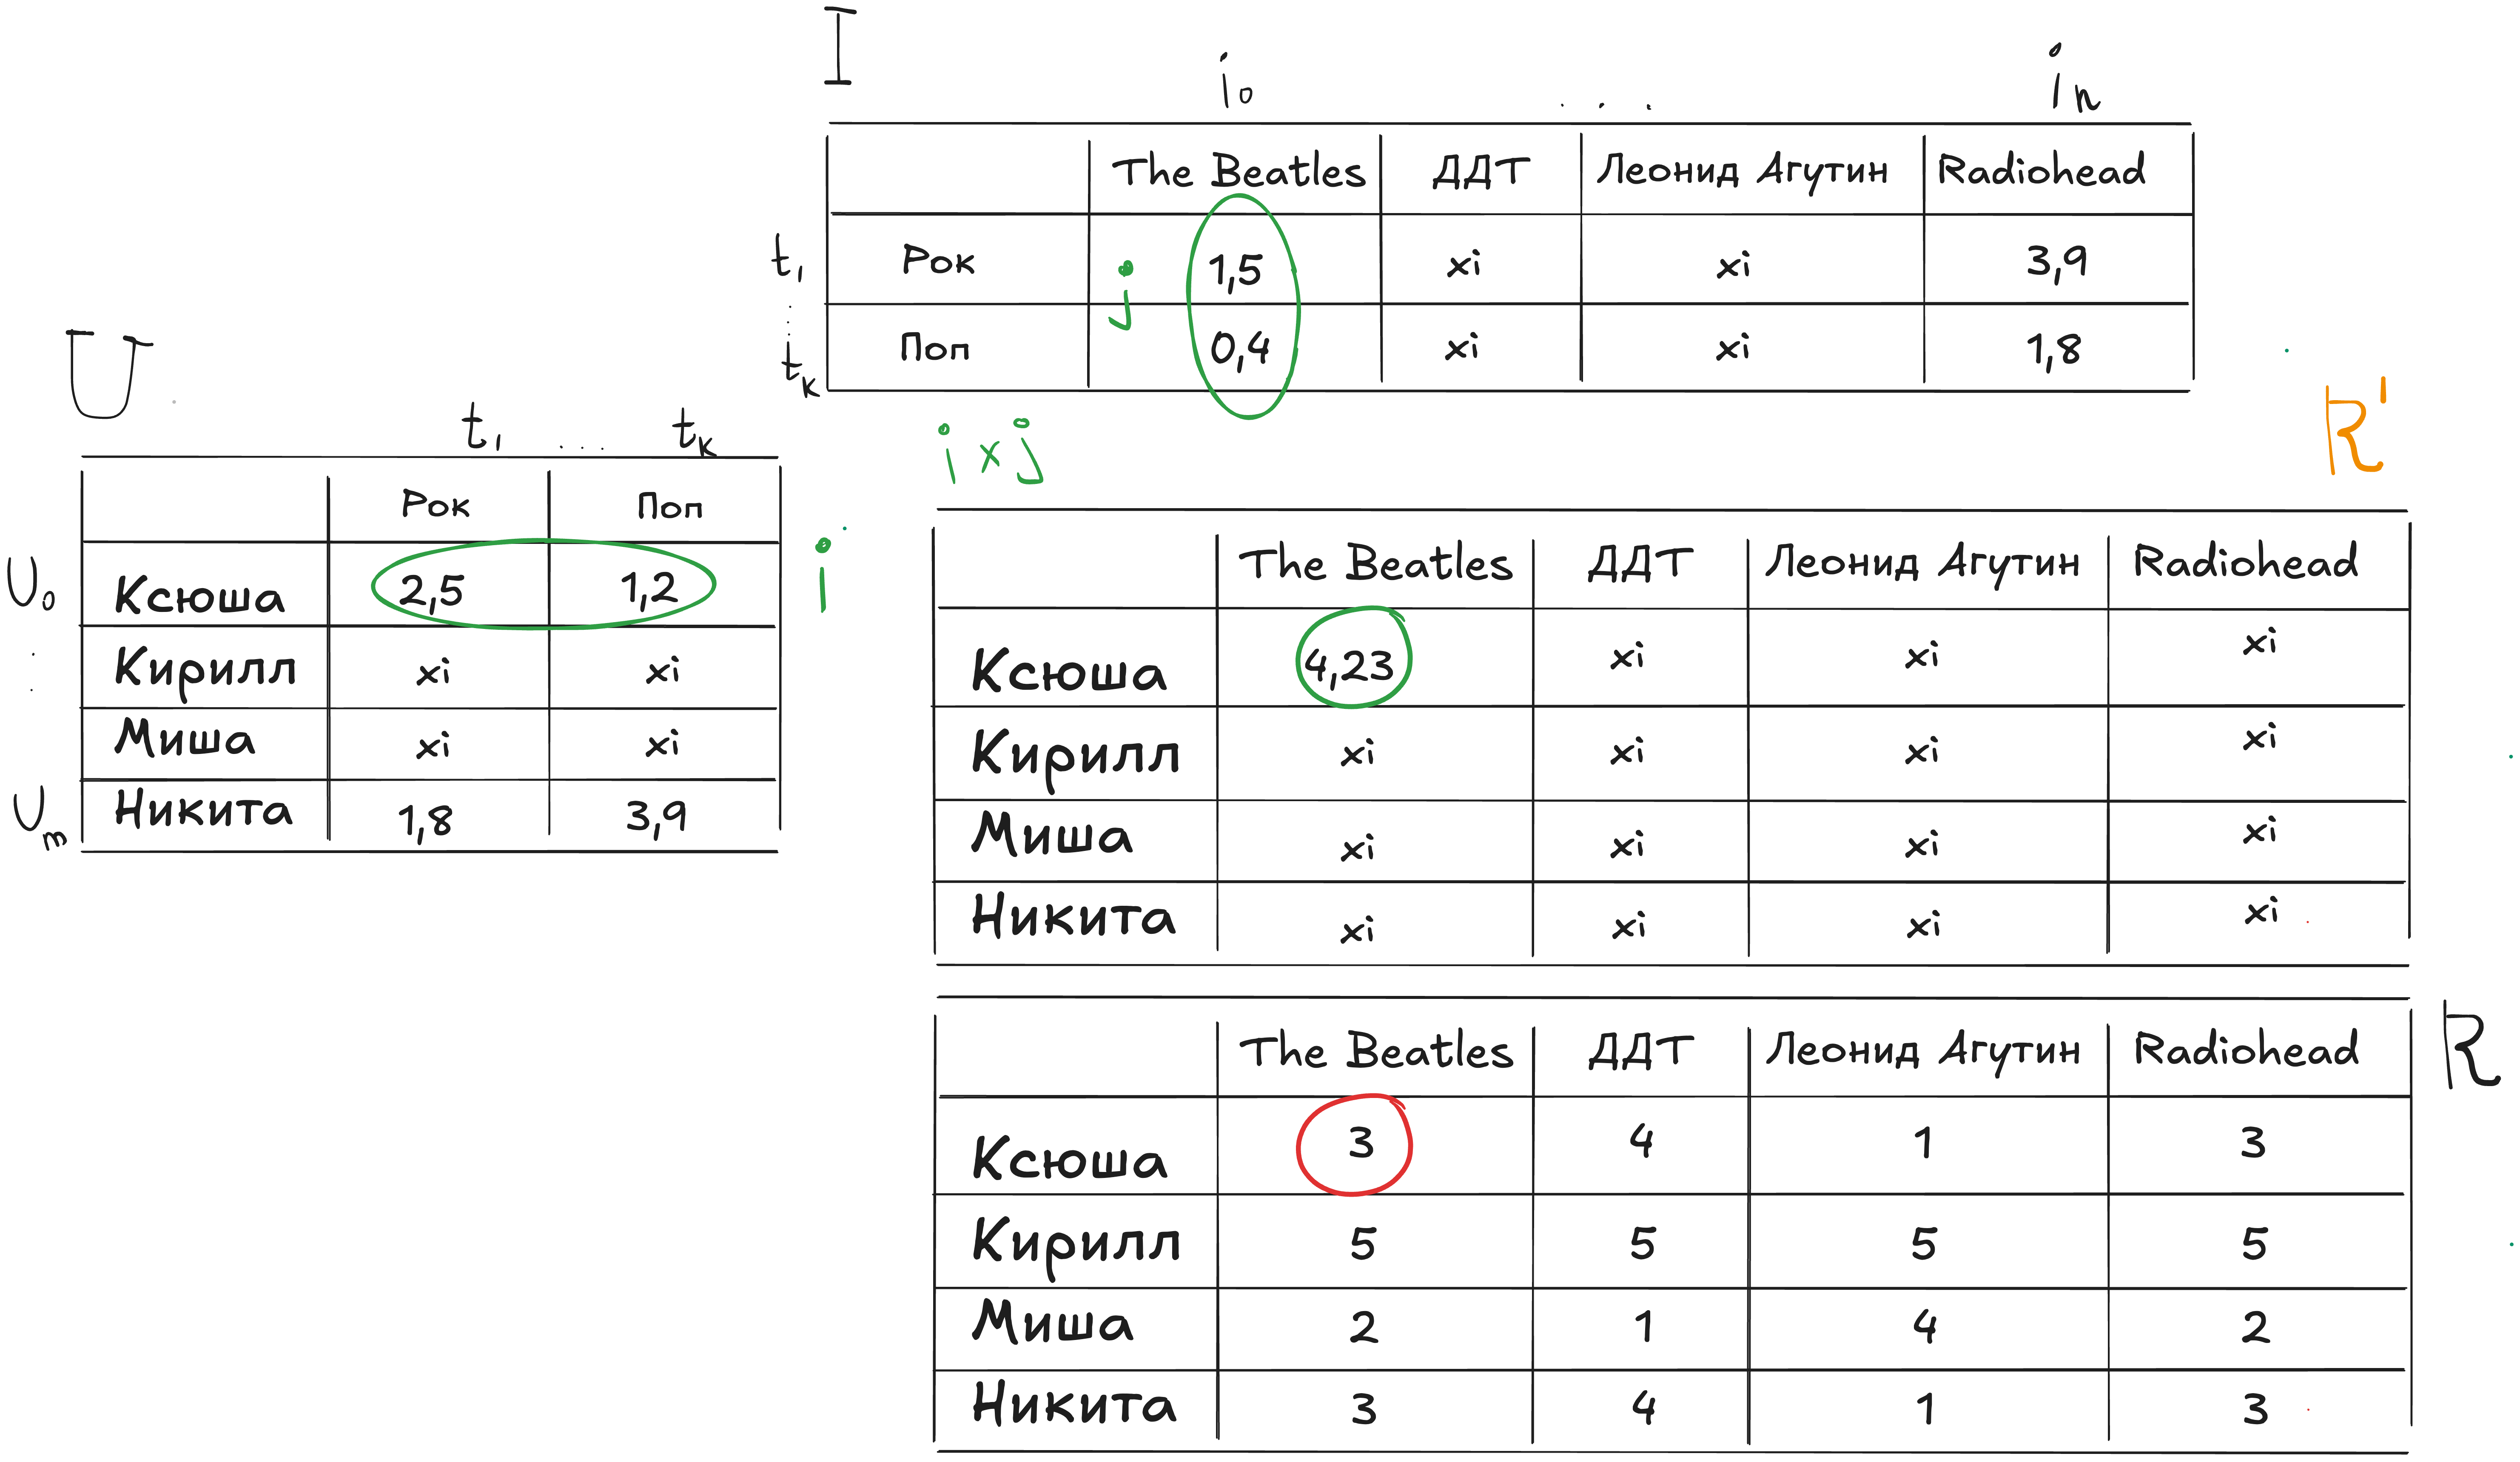
\includegraphics[width=1\textwidth]{./8.png}
  \caption{}
\end{figure}

% \begin{thebibliography}{3}
%   \bibitem{1}  
%   Смоленчук Татьяна Владимировна Метод коллаборативной фильтрации для рекомендательных сервисов // Вестник науки и образования. 2019. №22-1 (76). URL: https://cyberleninka.ru/article/n/metod-kollaborativnoy-filtratsii-dlya-rekomendatelnyh-servisov (дата обращения: 18.12.2024).
%   \bibitem{2}
%   Ларионов В. С., Дунин И. В. ОБЗОР МЕТОДОВ КОЛЛАБОРАТИВНОЙ ФИЛЬТРАЦИИ // Форум молодых ученых. 2017. №5 (9). URL: https://cyberleninka.ru/article/n/obzor-metodov-kollaborativnoy-filtratsii (дата обращения: 18.12.2024). 
%   \bibitem{3}
%   Гомзин А. Г., Коршунов А. В. Системы рекомендаций: обзор современных подходов // Труды ИСП РАН. 2012. №. URL: https://cyberleninka.ru/article/n/sistemy-rekomendatsiy-obzor-sovremennyh-podhodov (дата обращения: 18.12.2024).
%   \bibitem{4}
%  https://cts.etu.ru/assets/files/2021/cts21/papers/287-290.pdf

%  \bibitem{5}
%  https://education.yandex.ru/handbook/ml/article/intro-recsys
%  \bibitem{6}
%  http://www.machinelearning.ru/wiki/images/archive/9/95/20140413184117!Voron-ML-CF.pdf
% \end{thebibliography}

\bibliographystyle{ugost2003}
\bibliography{thesis}

\end{document}